\documentclass[border=10pt]{standalone}
\usepackage[svgnames]{xcolor}
\usepackage{amsmath}
\usepackage{pgfplots}
\pgfplotsset{compat=newest}
\usepackage[sfdefault]{FiraSans}
\usepackage{FiraMono}
\renewcommand*\familydefault{\sfdefault}
\begin{document}
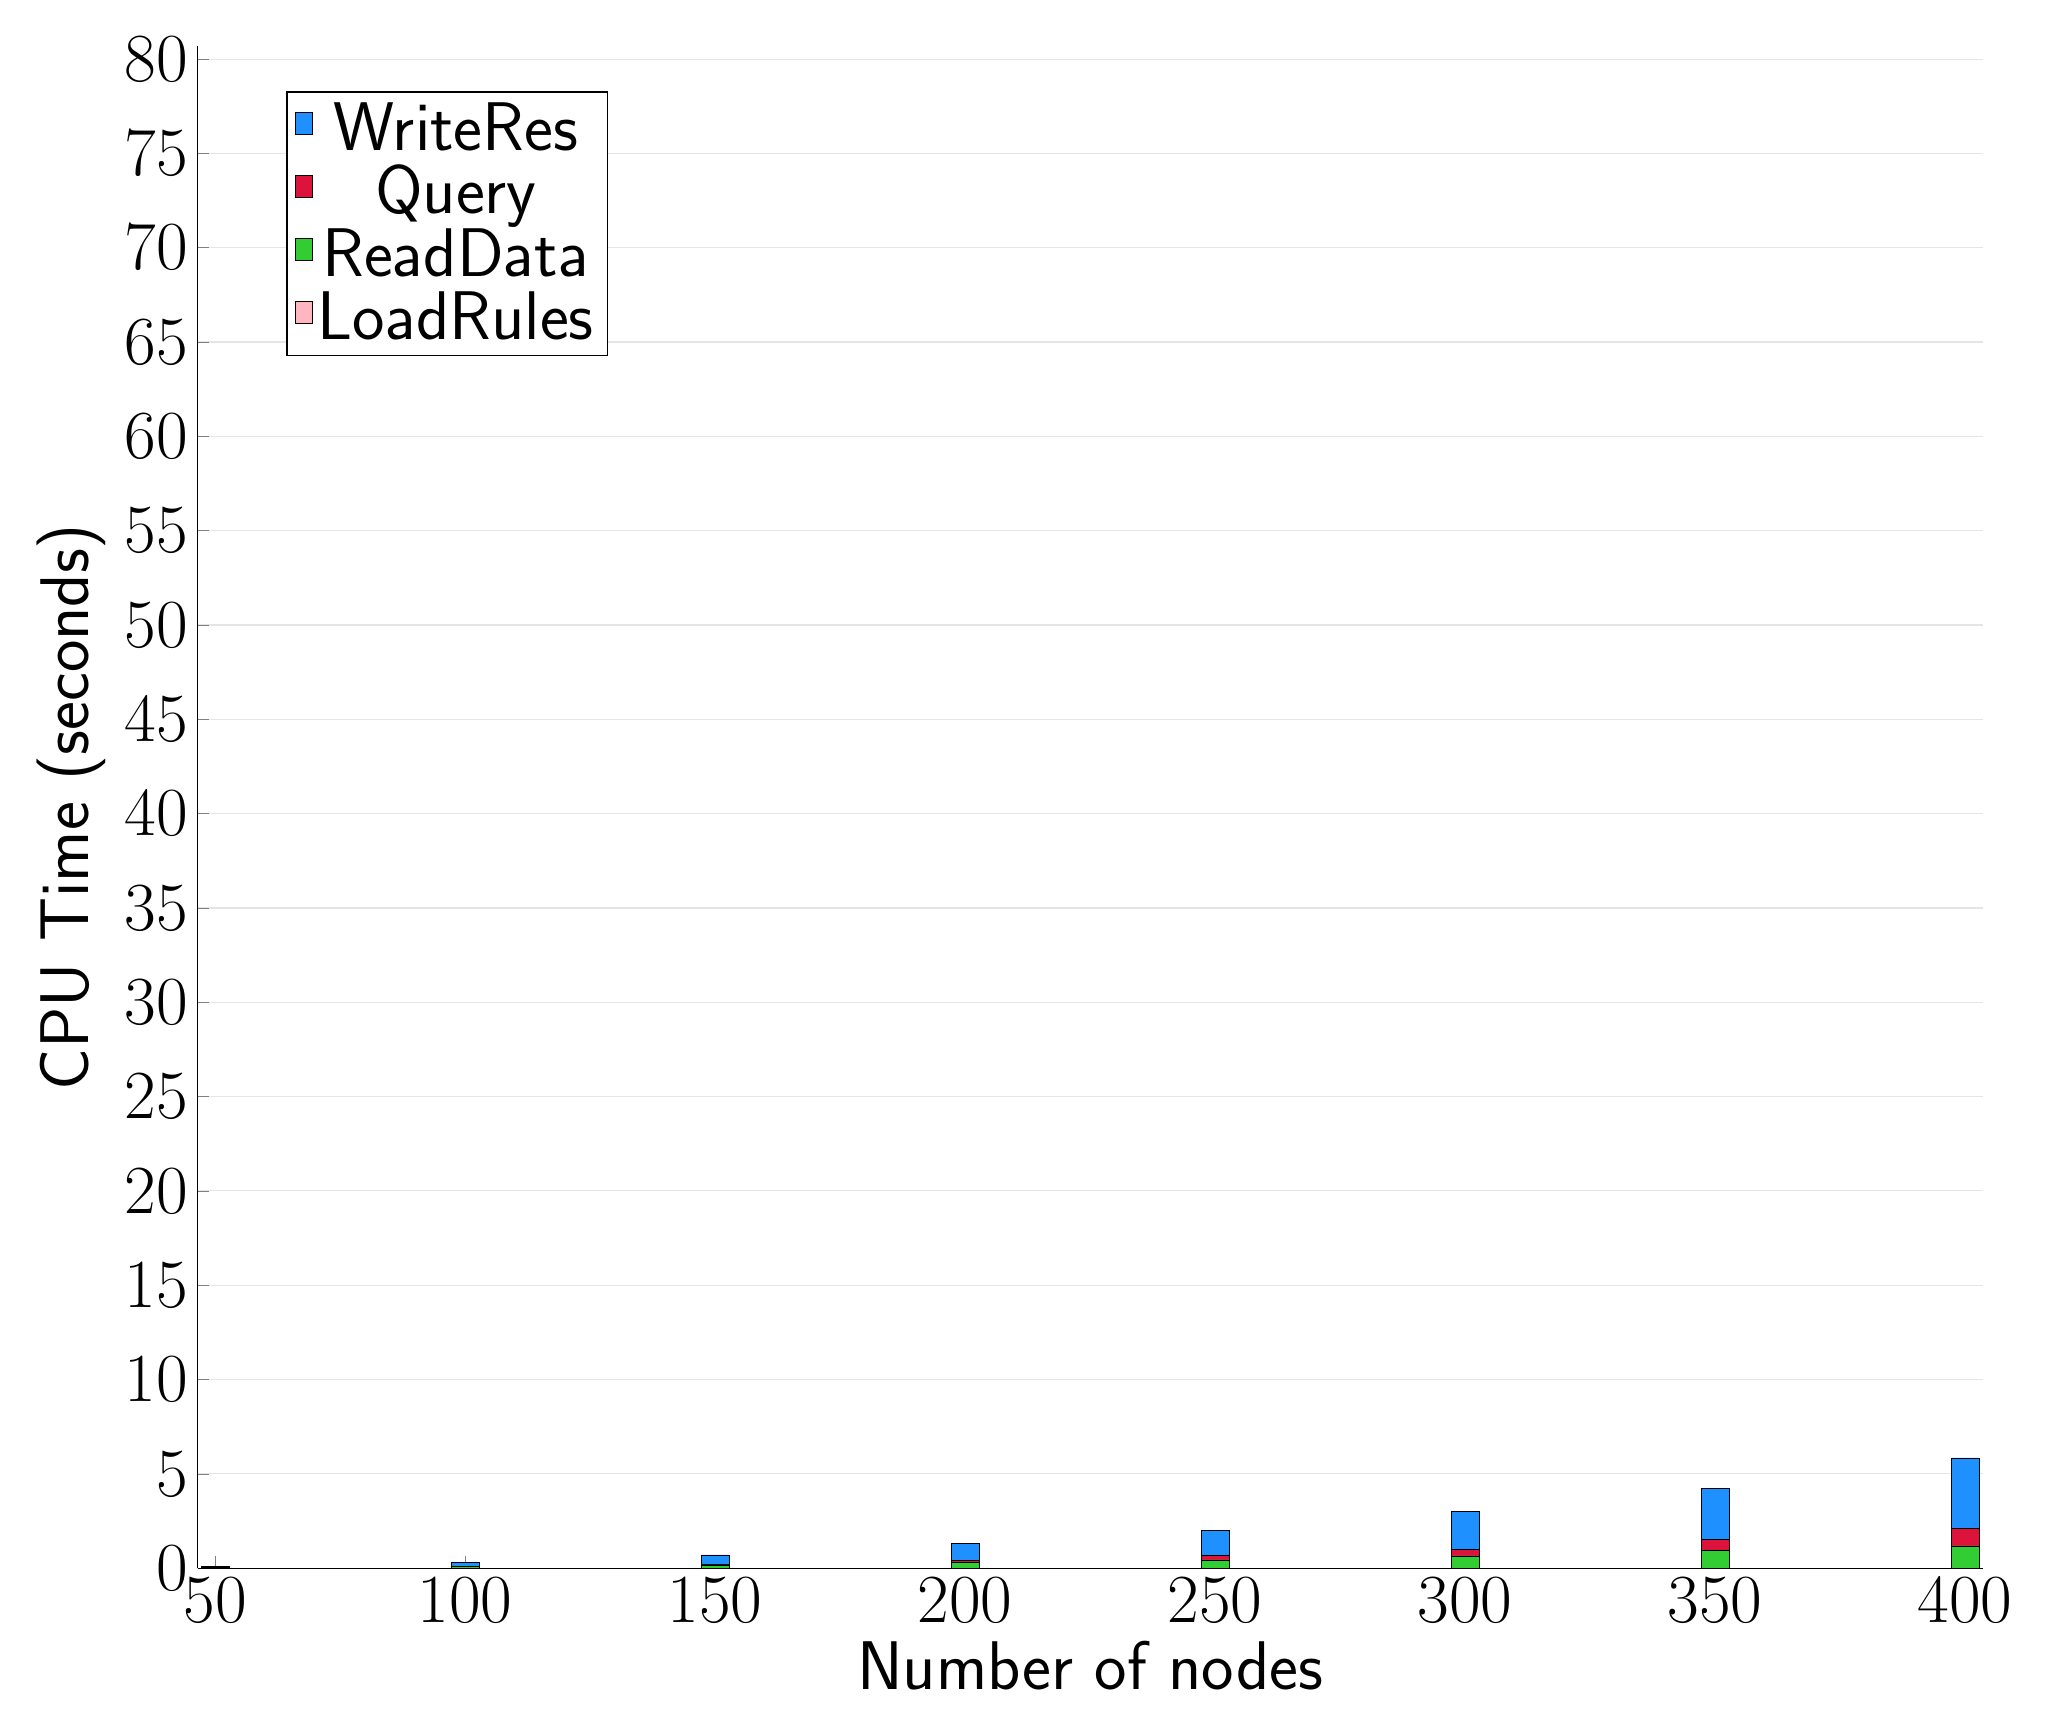
\begin{tikzpicture}
\begin{axis}[
   ybar stacked,
   width=2\textwidth,
   bar width=0.35cm,
   ymajorgrids, tick align=inside,
   major grid style={draw=gray!20},
   xtick=data,
   ymin=0, ymax=80.70666666577259,
   axis x line*=bottom,
   axis y line*=left,
   enlarge x limits=0.01,
   legend style={
       at={(0.23, 0.97)},
       anchor=north east,
       legend columns=1,
       font=\Huge,
   },
   ylabel={CPU Time (seconds)},
   xlabel={Number of nodes},
   label style={font=\Huge},
   tick label style={font=\Huge},
]
\addlegendimage{fill=DodgerBlue, draw=black, line width=0.2pt}
\addlegendentry{WriteRes}
\addlegendimage{fill=Crimson, draw=black, line width=0.2pt}
\addlegendentry{Query}
\addlegendimage{fill=LimeGreen, draw=black, line width=0.2pt}
\addlegendentry{ReadData}
\addlegendimage{fill=LightPink, draw=black, line width=0.2pt}
\addlegendentry{LoadRules}
\addplot +[fill=LightPink, draw=black, line width=0.2pt] coordinates {
(50, 0.004902999999999993)
(100, 0.0033386666666666656)
(150, 0.002721)
(200, 0.00474533333333333)
(250, 0.0024796666666666665)
(300, 0.0025319999999999995)
(350, 0.004824333333333333)
(400, 0.003636999999999999)
};
\addplot +[fill=LimeGreen, draw=black, line width=0.2pt] coordinates {
(50, 0.020528666666666667)
(100, 0.07371966666666667)
(150, 0.16701599999999997)
(200, 0.28599099999999994)
(250, 0.44164833333333336)
(300, 0.6452856666666666)
(350, 0.9189189999999999)
(400, 1.1824266666666665)
};
\addplot +[fill=Crimson, draw=black, line width=0.2pt] coordinates {
(50, 0.0025509999999999964)
(100, 0.017327)
(150, 0.04761066666666666)
(200, 0.10383533333333332)
(250, 0.2358293333333333)
(300, 0.349956)
(350, 0.5962506666666667)
(400, 0.934773)
};
\addplot +[fill=DodgerBlue, draw=black, line width=0.2pt] coordinates {
(50, 0.06061366666666667)
(100, 0.226429)
(150, 0.49321100000000007)
(200, 0.9246016666666668)
(250, 1.3086546666666665)
(300, 1.996117)
(350, 2.7057629999999997)
(400, 3.721864666666667)
};
\end{axis}
\end{tikzpicture}

\end{document}
